\begin{refsection}
\chapter{Statistical considerations}
\label{ch:statistics}

\section{The normal distribution}
\label{sec:Gauss}

Geochronological data processing is generally concerned with isotopic
ratio measurements, which are acquired by mass spectrometers and are
affected by random detector noise. Unless explicitly specified
otherwise, we will assume that this noise follows a Gaussian
distribution. In one dimension, this distribution is described by the
following probability density function (pdf):
\begin{equation}
  \mathcal{N}(x|\mu,\sigma^2) = \frac{1}{\sigma\sqrt{2\pi}}
  \exp\!\left[-\frac{(x-\mu)^2}{2\sigma^2}\right]
  \label{eq:gauss}
\end{equation}

\noindent where $\mu$ is the \textbf{mean} and $\sigma$ is the
\textbf{standard deviation}.

\begin{enumerate}
\item the \textbf{mean} $\mu$ controls the \textbf{location} of the
  distribution.
\item the \textbf{standard deviation} $\sigma$ quantifies the
  \textbf{dispersion} of the distribution.
\end{enumerate}

The interval from $\mu-\sigma$ to $\mu+\sigma$ covers 68.27\% of the
area under the PDF, and the interval from $\mu-2\sigma$ to
$\mu+2\sigma$ covers 95.45\%. Conversely 95\% of the area under the
normal PDF is contained within an interval of $\mu\pm{1.96}\sigma$.

\noindent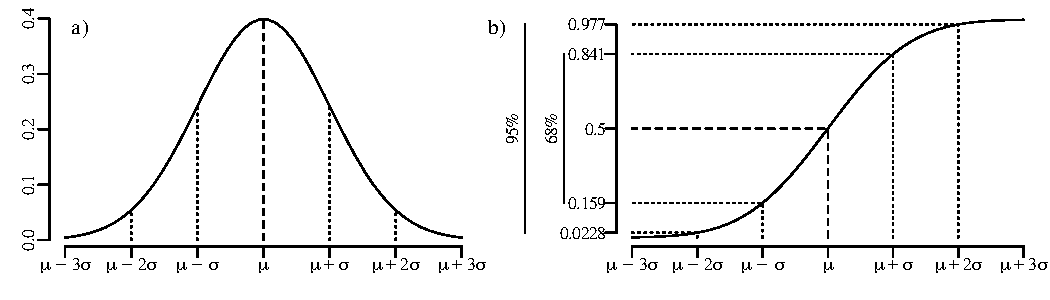
\includegraphics[width=\textwidth]{../figures/2sigma.pdf}
\begingroup \captionof{figure}{a) pdf and b) cumulative distribution
  fuction (cdf, i.e., the integral of the pdf) of the normal
  distribution.  The $\mu\pm\sigma$ and $\mu\pm{2}\sigma$ intervals
  cover $\sim$68\% and $\sim$95\% of the distribution,
  respectively.\\}
\label{fig:2sigma}
\endgroup

It can be mathematically proven that the \emph{sum} of $n$ randomly
selected values converges to a Gaussian distribution, provided that
$n$ is large enough. This convergence is guaranteed \textit{regardless
  of the distribution of the original data}.  This mathematical law is
called the \textbf{Central Limit Theorem}. Physically processes such
as thermal diffusion are characterised by white noise and Brownian
walks which are, in effect, additive processes.  So it makes sense
that these give rise to Gaussian distributions. In fact, these
additive processes are so common that the Gaussian distribution is
also known as the normal distibution, implying that all other
distributions are `abnormal'.\\

The normal distribution can be generalised to two dimensions using a
pdf that comprises five parameters: the means $\mu_x$ and $\mu_y$, the
standard deviations $\sigma_x$ and $\sigma_y$, and the covariance
$\sigma_{x,y}$:
\begin{equation}
\mathcal{N}(x,y|\mu_x,\mu_y,\sigma_x^2,\sigma_y^2,\sigma_{x,y}) = \frac{
\exp\left(-
\left[\begin{array}{@{}cc@{}}
(x-\mu_x) & (y-\mu_y)
\end{array}\right]
\left[\begin{array}{@{}c@{}c@{}}
\sigma^2_x & \sigma_{x,y}\\
\sigma_{x,y} & \sigma^2_y
\end{array}\right]^{-1}
\left[\begin{array}{@{}c@{}}
x-\mu_x\\
y-\mu_y
\end{array}\right] \biggl/ 2
\right)
}{2\pi\sqrt{
\left|\begin{array}{@{}c@{}c@{}}
\sigma^2_x & \sigma_{x,y}\\
\sigma_{x,y} & \sigma^2_y
\end{array}\right|
}}
\label{eq:2dgauss}
\end{equation}

\noindent where we recognise the \textbf{covariance matrix} as
\[\Sigma_{x,y} = 
\left[\begin{array}{@{}c@{}c@{}}
\sigma^2_x & \sigma_{x,y}\\
\sigma_{x,y} & \sigma^2_y
\end{array}\right]
\]

Finally, we can define the \textbf{correlation coefficient} as:
\begin{equation}
  \rho[x,y] \equiv \frac{s[x,y]}{\sqrt{s[x]s[y]}} 
  \approx 
  \frac{\sigma[x,y]}{\sqrt{\sigma[x]\sigma[y]}}
  \equiv \rho
  \label{eq:rho}
\end{equation}

\noindent $\rho[x,y]$ is akin to a normalised covariance, whose values
range from $-1$ (perfect negative correlation) to $+1$ (perfect
positive correlation).

\section{The method of maximum likelihood}
\label{sec:maximum-likelihood}

The parameters $\mu$ and $\sigma$ of the normal distribution are
\emph{unknown} but can be \emph{estimated} from the data. This can be
done using the \textbf{method of maximum likelihood}.  Given $n$ data
points $\{x_1, x_2, \ldots, x_n\}$ drawn from a normal distribution,
we can formulate the normal likelihood function as
\begin{equation}
  \mathcal{L}(\mu,\sigma^2|x_1,x_2,\ldots,x_n) =
  \prod\limits_{i=1}^{n}\mathcal{N}(x_i|\mu,\sigma^2)
  \label{eq:Lnorm}
\end{equation}

$\mu$ and $\sigma$ can be estimated by maximising the likelihood or,
equivalently, the log-likelihood:
\begin{equation}
  \begin{split}
    \mathcal{LL}(\mu,\sigma^2|x_1,x_2,\ldots,x_n) & =
    \sum\limits_{i=1}^{n}\ln\left[\mathcal{N}(x_i|\mu,\sigma^2)\right] \\ & =
    \sum\limits_{i=1}^{n} -\ln[\sigma] - \frac{1}{2}\ln[2\pi] -
    \frac{(x_i-\mu)^2}{2\sigma^2}
  \end{split}
  \label{eq:LLnorm}
\end{equation}

Taking the derivative of $\mathcal{LL}$ with respect to $\mu$ and
setting it to zero:
\begin{equation}
  \begin{split}
    \frac{\partial{\mathcal{LL}}}{\partial{\mu}} & =
    - \sum\limits_{i=1}^{n} \frac{x_i-\mu}{\sigma^2} = 0 \\
    & \Rightarrow n\mu - \sum\limits_{i=1}^{n} x_i = 0 \\
    & \Rightarrow \bar{x} = \frac{1}{n}\sum\limits_{i=1}^{n}x_i
  \end{split}
  \label{eq:arithmeticmean}
\end{equation}

\noindent which is the same as Equation~\ref{eq:mean}. Using the same
strategy to estimate $\sigma$:
\begin{equation}
  \begin{split}
    \frac{\partial{\mathcal{LL}}}{\partial{\sigma}} & =
    \sum\limits_{i=1}^{n} - \frac{1}{\sigma} +  \frac{(x_i-\mu)^2}{\sigma^3} = 0\\
    & \Rightarrow  \sum\limits_{i=1}^{n} \frac{(x_i-\mu)^2}{\sigma^3} =
    \frac{n}{\sigma} \\
    & \Rightarrow \hat{\sigma} = \sqrt{\frac{1}{n}\sum\limits_{i=1}^{n}(x_i-\mu)^2}
  \end{split}
  \label{eq:stdevgivenmu}
\end{equation}

\noindent which is nearly identical to the formula for the standard
deviation that we saw in Section~\ref{sec:summarystatistics}:
\begin{equation}
  s[x] = \sqrt{\frac{1}{n-1}\sum\limits_{i=1}^{n}(x_i-\bar{x})^2}
  \label{eq:stdev}
\end{equation}

There are just two differences between
Equations~\ref{eq:stdev} and
Equation~\ref{eq:stdevgivenmu}:
\begin{enumerate}
\item Equation~\ref{eq:stdevgivenmu} uses the population mean $\mu$,
  whereas Equation~\ref{eq:stdev} uses the sample mean $\bar{x}$.
\item Equation~\ref{eq:stdevgivenmu} divides the sum of the squared
  differences between the measurements and the mean by $n$, whereas
  Equation~\ref{eq:stdev} divides it by ($n-1$).
\end{enumerate}

The two differences are related to each other. The subtraction of 1
from $n$ is called the \textbf{Bessel correction} and accounts for the
fact that by using an estimate of the mean ($\bar{x}$), rather than
the true value of the mean ($\mu$), we introduce an additional source
of uncertainty in the estimate of the standard deviation. This
additional uncertainty is accounted for by subtracting one
\textbf{degree of freedom} from the model fit.\\

Again using the method of maximum likelihood, it is possible to
estimate the covariance for bivariate normal distributions as (proof
omitted):
\begin{equation}
  \hat{\sigma}_{x,y} = \sum\limits_{i=1}^{n}\frac{1}{n}(x_i-\mu_x)(y_i-\mu_y)
\end{equation}

\noindent or, if $\mu_x$ and $\mu_y$ are unknown and must be estimated
from the data as well:
\begin{equation}
  s[x,y] = \sum\limits_{i=1}^{n}\frac{1}{n-1}(x_i-\bar{x})(y_i-\bar{y})
  \label{eq:sxy}
\end{equation}

Thus we can estimate the \textbf{covariance matrix}
(Equation~\ref{eq:s2tmatrix}) of the bivariate normal distribution as:
\begin{equation}
  \Sigma_{x,y} =
  \left[
    \begin{array}{@{}c@{~}c@{}}
      s[x]^2 & s[x,y]\\
      s[x,y] & s[y]^2
    \end{array}
    \right]
\end{equation}

Finally, we can define the \textbf{correlation coefficient} as:
\begin{equation}
  r \equiv \frac{s[x,y]}{\sqrt{s[x]s[y]}} 
  \approx 
  \frac{\sigma[x,y]}{\sqrt{\sigma[x]\sigma[y]}}
  \equiv \rho
  \label{eq:r}
\end{equation}

Besides providing a powerful tool to estimate parameters from data,
the method of maximum likelihood can also be used to estimate the
standard errors of those parameters. Let $\hat{z}$ be the maximum
likelihood estimate of some parameter $z$. We can approximate the
log-likelihood with a second order Taylor series in the vicinity of
$\hat{z}$:
\[
  \mathcal{LL}(z) \approx \mathcal{LL}(\hat{z}) +
  \frac{\partial\mathcal{LL}}{\partial{z}} (z-\hat{z}) +
  \frac{1}{2} \frac{\partial^2\mathcal{LL}}{\partial{z^2}} (z-\hat{z})^2
\]

By definition, $\partial{\mathcal{LL}}/\partial{z}=0$ at
$\hat{z}$. Therefore, the likelihood ($\mathcal{L}(z) =
\exp[\mathcal{LL}(z)]$) is proportional to:
\[
\mathcal{L}(z) \propto 
\exp\left[
  \frac{1}{2} \frac{\partial^2\mathcal{LL}}{\partial{z^2}} (z-\hat{z})^2
  \right]
\]

\noindent which can also be written as:
\[
\mathcal{L}(z) \propto \exp\!\left[
  -\frac{1}{2} \frac{(z-\hat{z})^2}{
    -\frac{1}{\frac{\partial^2\mathcal{LL}}{\partial{z^2}}}
  }\right]
\]

This equation fits the functional form of the normal distribution
(Equation~\ref{eq:gauss}):
\[
\mathcal{L}(z) \propto \exp\!\left[
  -\frac{1}{2} \frac{(z-\hat{z})^2}{\sigma[z]^2}
  \right]
\]

\noindent which leads to
\begin{equation}
  \sigma[z]^2 = \frac{1}{-\frac{\partial^2\mathcal{LL}}{\partial{z^2}}}
  \label{eq:Fisher}
\end{equation}

$-\frac{\partial^2\mathcal{LL}}{\partial{z^2}}$ is known as the
\textbf{Fisher Information}. Equation~\ref{eq:Fisher} can be
generalised to multiple dimensions:
\begin{equation}
  \Sigma = -\mathcal{H}^{-1}
  \label{eq:multidimFisher}
\end{equation}

\noindent where $\Sigma$ is the covariance matrix and
$(\mathcal{H})^{-1}$ is the inverse of the (`Hessian') matrix of
second derivatives of the log-likelihood function with respect to the
parameters.

\section{The mean square of weighted deviates (MSWD)}
\label{sec:mswd}

Let $t = \{t_1, \ldots, t_n\}$ be a set of $n$ age estimates
determined on different aliquots of the same sample with a true age
$\mu[t]$, and let $\sigma[t] = \sigma[t_1] = \ldots = \sigma[t_n]$ be
their normally distributed analytical uncertainty. Then we can
estimate $\mu[t]$ and $\sigma[t]$ with
Equations~\ref{eq:arithmeticmean} and \ref{eq:stdev}, respectively.
However, if each of the $n$ age estimates has its own analytical
uncertainty ($\sigma[t_1] \neq \ldots \neq, \sigma[t_n]$), then it is
important to account for this \textit{heteroscedasticity}. Consider,
for example, the following dataset of four samples:

\begin{center}
\begin{tabular}{c|ccccc}
  $i$ & 1 & 2 & 3 & 4 \\
$t_i$ & 1005 & 1000 & 995 & 1125 \\
$s[t_i]$ & 10 & 10 & 10 & 100
\end{tabular}
\captionof{table}{Heteroscedastic dataset of four age estimates (in Ma).}
\label{tab:wtdmean}
\end{center}

Then the arithmetic mean is 1031~Ma, which plots outside the 95\%
confidence intervals of all three of the four aliquots. The
\textbf{error weighted mean} addresses this issue:
\begin{equation}
  \bar{t}_w = \frac{\sum_{i=1}^n (t_i/s[t_i]^2) }{\sum_{i=1}^n (1/s[t_i]^2) }
  \label{eq:wtdmean}
\end{equation}

Applying Equation~\ref{eq:wtdmean} to the example dataset attaches a
smaller weight to the imprecise fourth measurement, yielding a
$\bar{t}_w$ value of 1000.4~Ma:

\noindent\begin{minipage}[t]{.5\textwidth}
\strut\vspace*{-\baselineskip}\newline
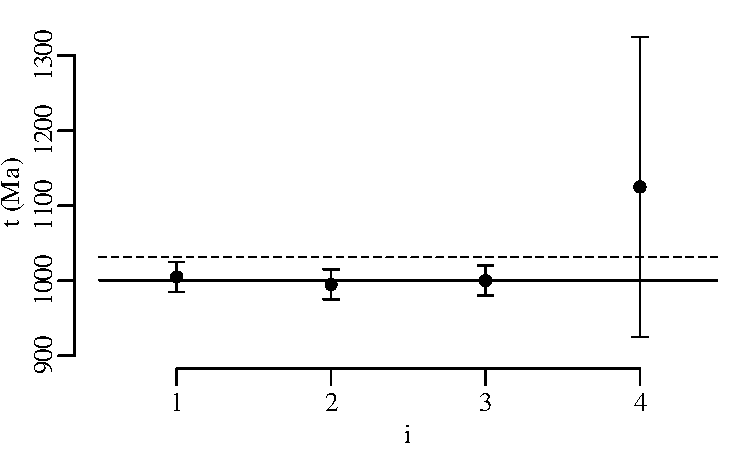
\includegraphics[width=\textwidth]{../figures/wtdmean.pdf}
\end{minipage}
\begin{minipage}[t]{.5\textwidth}
  \captionof{figure}{ The data of Table~\ref{tab:wtdmean} with 95\%
    confidence intervals shown as error bars, the weighted mean as a
    dashed horizontal line and the error weighted mean as a solid
    line.}
  \label{fig:wtdmean}
\end{minipage}

The extent to which the observed scatter in the data around the
weighted mean can be explained by the analytical uncertainties can be
assessed using a chi-square test.  To this end, we define the
chi-square statistic as:
\begin{equation}
  \chi^2_{stat} = \sum\limits_{i=1}^{n}\frac{(t_i-\bar{t}_w)^2}{s[t_i]^2}
  \label{eq:chi2wtdmean}
\end{equation}

For the data of Table~\ref{tab:wtdmean}:
\[
\chi^2_{stat} = \frac{(1005-1000.4)^2}{10^2}
+ \frac{(1000-1000.4)^2}{10^2}
+ \frac{(995-1000.4)^2}{10^2} +
\frac{(1125-1000.4)^2}{100^2}
= 2.06
\]
  
We can compare this value with a chi-square distribution with $df = n
- 1$ degrees of freedom. In the case of the example dataset, $n=4$ and
$df=3$. The \textbf{p-value} is defined as the probability of
observing a value greater than $\chi_{stat}^2$ under this
distribution:

\noindent\begin{minipage}[t]{.7\textwidth}
\strut\vspace*{-\baselineskip}\newline
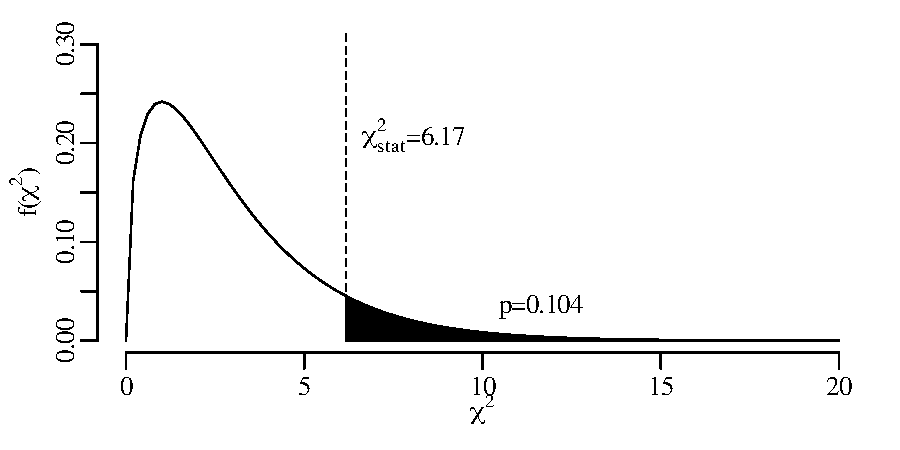
\includegraphics[width=\textwidth]{../figures/chi2wtdmean.pdf}
\end{minipage}
\begin{minipage}[t]{.3\textwidth}
  \captionof{figure}{Chi-square distribution with 3 degrees of
    freedom.  The p-value for an outcome of $\chi_{stat}^2=2.06$ is
    the integral of the black area.}
  \label{fig:chi2}
\end{minipage}

A cutoff of $\alpha=0.05$ is often used to assess whether the observed
scatter of the data around the weighted mean can be accounted for by
the analytical uncertainty alone.  For the example dataset, the
p-value is 0.561, which is greater than this \textbf{significance
  level}. Therefore, we have no reason to suspect that there are any
other sources of dispersion in the data besides analytical
uncertainty.\\

An alternative way to assess the data scatter is by dividing the
chi-square statistic $\chi^2_{stat}$ by the number of degrees of
freedom $df$.  The resulting numerical value is called the `Mean
Square of the Weighted Deviates' \citep[MSWD,][]{mcintyre1966} by
geochronologists, but is known as the `reduced chi-square statistic'
elsewhere.
\begin{equation}
  MSWD = \frac{\chi^2_{stat}}{n-1}
  \label{eq:mswd}
\end{equation}

For sufficiently large samples and, hence, degrees of
freedom, the distribution of the MSWD statistic converges to a normal
distribution with a mean of 1. However for small samples there is a
comparatively greater probability of obtaining an MSWD value that is
greater or smaller than 1:

\noindent\begin{minipage}[t]{.7\textwidth}
\strut\vspace*{-\baselineskip}\newline
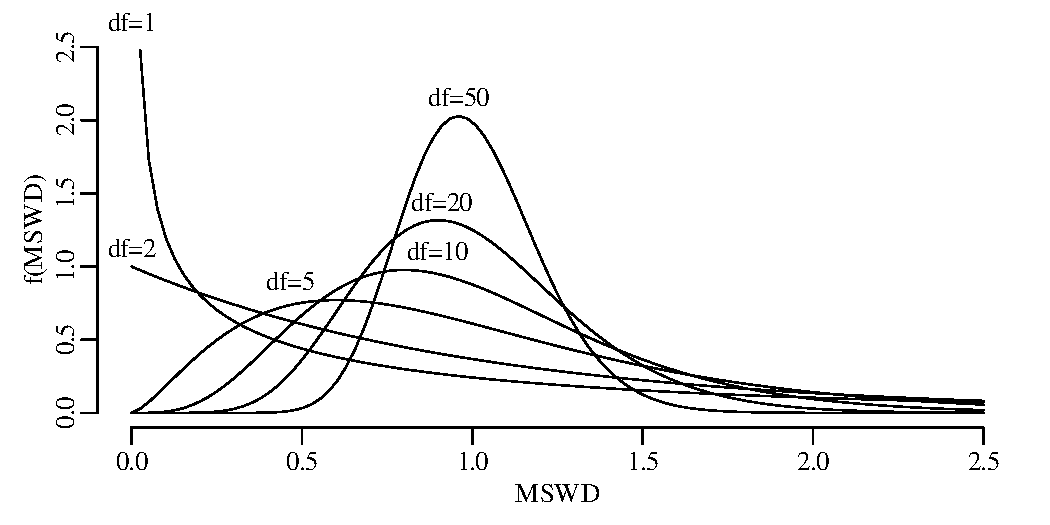
\includegraphics[width=\textwidth]{../figures/mswd.pdf}
\end{minipage}
\begin{minipage}[t]{.3\textwidth}
  \captionof{figure}{Expected distribution of the MSWD for different
    degrees of freedom. With increasing sample size, the distribution
    of the MSWD converges to a normal distribution with mean 1.}
  \label{fig:mswd}
\end{minipage}

The MSWD is a very useful device to assess the degree to which the
observed scatter of the data around the best fit can be explained by
the analytical uncertainties. Three scenarios are possible:

\begin{enumerate}
  \item If the analytical uncertainties alone explain the total
    scatter around the true mean, then the MSWD is expected to take on
    a value of $\approx{1}$.
\item Data sets that exhibit MSWD values close to zero are said to be
  ``underdispersed'' with respect to the analytical
  uncertainties. This indicates some problem with the error
  propagation, which is often due to undetected systematic effects.
\item Finally, MSWD values $>1$ can often be attributed to some form
  of geological dispersion. This overdispersion carries geological
  significance.
\end{enumerate}

\noindent\begin{minipage}[t]{.4\textwidth}
\strut\vspace*{-\baselineskip}\newline
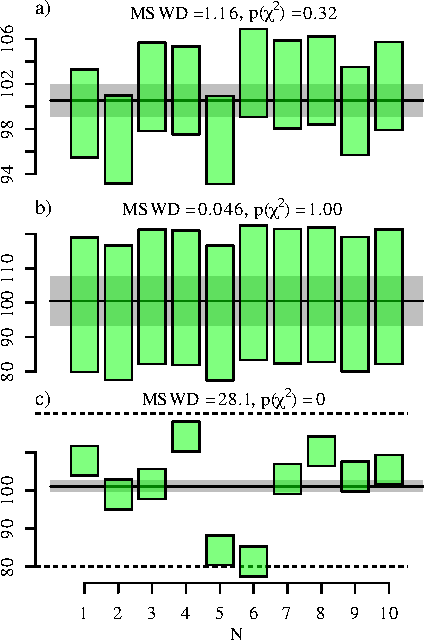
\includegraphics[width=\textwidth]{../figures/wtdmeanMSWD.pdf}
\end{minipage}
\begin{minipage}[t]{.02\textwidth}
~
\end{minipage}
\begin{minipage}[t]{.58\textwidth}
  \captionof{figure}{Three different synthetic data sets shown as
    weighted mean plots. The analytical uncertainties are shown as
    95\% error bars. Each of the data sets consists of 10 aliquots
    that are affected by a combination of analytical and geological
    dispersion. The relative importance of these two sources of
    scatter can be assessed using the mean square of weighted deviates
    (MSWD) and the p-value of the chi-square test. The case where
    MSWD$\approx{1}$ is the easiest to interpret: it means that the
    scatter of the data around the best fit line can be completely
    explained by the analytical uncertainty. The case where MSWD$<{1}$
    may seem like a good outcome but it is in fact a bad one because
    it indicates that there may be a problem with the error
    propagation. A high p-value or low MSWD may happen once but red
    flags should go up if all samples in a study show this type of
    behaviour. Finally the case where MSWD$>{1}$ is not good or bad
    but `interesting'. The dashed lines mark the 95\% confidence
    limits of a normal distribution whose mean equals the weighted
    mean age, and whose standard deviation is given by the
    overdispersion parameter ($\omega=10$~Ma) as discussed in
    Section~\ref{sec:overdispersion}.}
  \label{fig:wtdmeanMSWD}
\end{minipage}

\section{Dealing with overdispersion}
\label{sec:overdispersion}

\texttt{IsoplotR} offers three strategies (`models') to deal with
overdispersed datasets:

\begin{enumerate}
\item\textbf{Model-1: inflate the analytical uncertainties until MSWD=1}

  A `model-1' average assumes that the overdispersion of the data is due
  to an underestimation of the analytical uncertainties by a common
  factor $f$. To `fix' the overdispersion, the model-1 fit simply
  multiplies the uncertainties with this number and plugs the resulting
  value into Equation~\ref{eq:mswd}:
  \[
  \sum\limits_{i=1}^{n}\frac{(t_i-\bar{t}_w)^2}{(n-1) (f~s[t_i])^2} = 1
  \Rightarrow f = \sqrt{MSWD}
  \]

\item\textbf{Model-2: ignore the analytical uncertainties}
  
  Although the $\sqrt{MSWD}$ trick is attractive from a mathematical
  point of view, the physical meaning of the overdispersion factor is
  not always clear. It effectively means that the reported analytical
  uncertainties are not reliable. But if this is the case, then one
  might wonder why the degree of unreliability should be the same
  (i.e. a factor of $\sqrt{MSWD}$) for all aliquots. An alternative
  way to deal with unreliable uncertainty estimates is to ignore them
  altogether and use the ordinary arithmetic mean as a fallback
  solution.
  
\item\textbf{Model-3: quantify the overdispersion}

  The most sophisticated, and arguable most realistic method to deal
  with overdispersed dataset is to attribute them to geological
  effects. A `model-3' weighted mean assumes that the data were drawn
  from a normal distribution with two sources of variance:
  \begin{equation}
    \mathcal{N}(x|\mu,\sigma^2+\omega^2) =
    \frac{1}{\sqrt{2\pi\left(\sigma^2+\omega^2\right)}}
    \exp\!\left[-\frac{(x-\mu)^2}{2\left(\sigma^2 + \omega^2 \right)}\right]
    \label{eq:overdispersion}
  \end{equation}

\noindent where $\omega$ is the \textbf{overdispersion}. $\mu$ and
$\omega$ can be estimated by maximising the following log-likelihood
function:
  \begin{equation}
    \mathcal{LL}_w \propto \sum\limits_{i=1}^{n}
    - \frac{1}{2}\ln\!\left(s[t_i]^2+\omega^2\right)
    + \left[-\frac{(x-\mu)^2}{2\left(s[t_i]^2 + \omega^2 \right)}\right]
    \label{eq:wtdmean-model-3}
  \end{equation}

In mathematical terms, model-3 is known as a \textbf{random effects
  model}. The overdispersion $\omega$ has physical meaning and may be
as useful as the mean age itself. Consider, for example, a batholith
whose emplacement age is determined by TIMS U--Pb geochronology of
igneous zircon. The analytical precision of TIMS measurements is on
the order of a few \textperthousand. So if the batholith was intruded
at 20~Ma, then the zircon ages can be determined to within 20ka. Large
intrusions often take much longer than 20kyr to crystallise. Therefore
it is unlikely that all the zircons have exactly the same age.  The
resulting geological dispersion will cause high MSWD values.  The
$\omega$ parameter of a model-3 weighted mean would quantify this
dispersion and thereby estimate the residence time of zircon in the
magma chamber.

\end{enumerate}

\section{Error correlations}
\label{sec:errorcorrelations}

Consider the generic age equation for a radioactive parent $P$
that decays to a radiogenic daughter $D$ in the presence of
an inherited component that can be traced by normalising to
a non-radiogenic isotope $d$ of the daughter element:
\begin{equation}
  t = \frac{1}{\lambda}
  \ln\left(\frac{\left[{D}/{d}\right]-\left[{D}/{d}\right]_\circ}
          {\left[{P}/{d}\right]} - 1\right)
\end{equation}

For example, $P$, $D$ and $d$ might be \textsuperscript{87}Rb,
\textsuperscript{87}Sr and \textsuperscript{86}Sr for Rb--Sr
geochronology, or \textsuperscript{238}U, \textsuperscript{206}Pb and
\textsuperscript{204}Pb for U--Pb
geochronology. Chapter~\ref{ch:error-propagation} showed that error
propagation of the age $t$ requires the characterisation of the full
covariance structure of the isotopic ratio data including their mean
values, their standard errors and their covariances or error
correlations. This covariance structure is estimated from the raw mass
spectrometer data using the low level data processing software
mentioned in Chapter~\ref{ch:intro2}.  The error propagation of
isotopic ratio data could be greatly simplified if the covariances
were negligible. Unfortunately this is generally not the case.  To
prove this point, consider the following set of synthetic mass
spectrometer data:\\

\noindent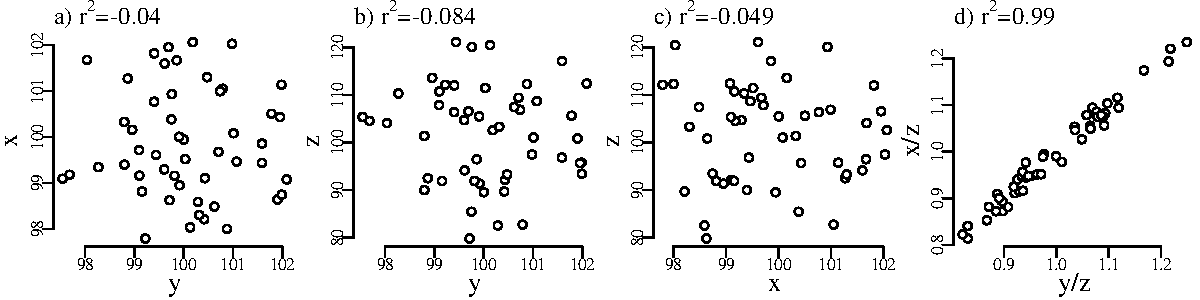
\includegraphics[width=\textwidth]{../figures/spurious}\\

\noindent where $x$, $y$ and $z$ are uncorrelated (normally
distributed) random numbers, but the ratios $y/z$ and $x/z$ are
strongly correlated. The \emph{spurious correlation} between ratios
like this was first described by \citet{pearson1896}. It is strongest
when the common nuclide $z$ is measured less precisely than the
remaining two nuclides $x$ and $y$. If the summary statistics of $x$,
$y$ and $z$ are known, then it is possible to predict the correlation
coefficient:

\begin{equation}
  \noindent r\left[\frac{y}{z},\frac{x}{z}\right] \approx
  \frac{
    \left({s[z]}/{z}\right)^2
  }{
    \sqrt{\left({s[x]}/{x}\right)^2 +
      \left({s[z]}/{z}\right)^2}
    \sqrt{\left({s[y]}/{y}\right)^2 +
      \left({s[z]}/{z}\right)^2}
  }
  \label{eq:spurious-conventional}
\end{equation}

For example, consider the following hypothetical Re--Os abundance
estimates:
\[
y = {}^{187}\mbox{Os} = 2,000 \pm 10 \mbox{~fmol;~}
x = {}^{187}\mbox{Re} = 30,000 \pm 100 \mbox{~fmol}
\mbox{~and~}
z = {}^{188}\mbox{Os} = 200 \pm 2 \mbox{~fmol}
\]

\noindent then the (\textsuperscript{187}Os/\textsuperscript{188}Os)
and (\textsuperscript{187}Re/\textsuperscript{188}Os) isotope ratio
estimates exhibit a correlation coefficient of
\[
  \noindent r\left[\frac{{}^{187}\mbox{Os}}{{}^{188}\mbox{Os}},
                   \frac{{}^{187}\mbox{Re}}{{}^{188}\mbox{Os}}\right]
  =
  \frac{
    \left(\frac{2}{200}\right)^2
  }{
    \sqrt{\left(\frac{100}{30,000}\right)^2 +
      \left(\frac{2}{200}\right)^2}
    \sqrt{\left(\frac{10}{2,000}\right)^2 +
      \left(\frac{2}{200}\right)^2}
  }
  = 0.85
\]

The strong error correlation between the two variables on the Re--Os
isochron diagram are manifested as narrow and steeply inclined error
ellipses. The same phenomenon manifests itself in all isotopic ratio
data to a lesser or greater degree:

\noindent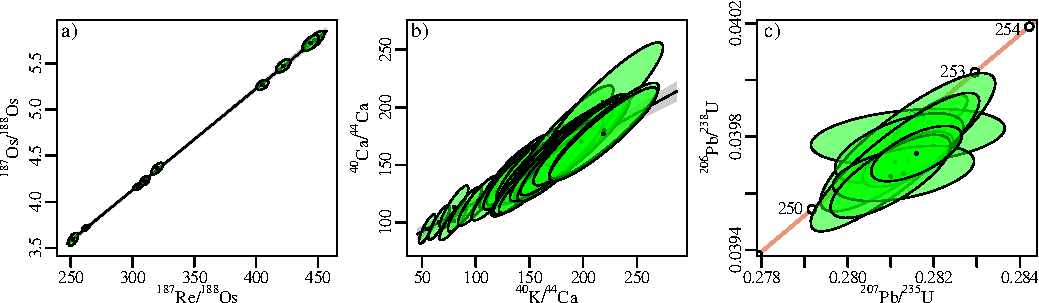
\includegraphics[width=\textwidth]{../figures/errorcorrelation_edited.pdf}
\begingroup
\captionof{figure}{ Examples of correlated uncertainties shown as
  confidence ellipses in a) Re--Os and b) K--Ca isochron and c)
  Wetherill U--Pb concordia space.\\}
\label{fig:errorcorrelation}
\endgroup

For some geochronometers, the error correlations can be reduced by
recasting the isotopes into two new ratios $z/y$ vs. $x/y$. If $y$ is
measured more precisely than $x$ and $z$, then this reduces the
spurious correlation coefficient. For example, revisiting the earlier
Re--Os example:
\[
  \noindent r\left[\frac{{}^{188}\mbox{Os}}{{}^{187}\mbox{Os}},
                   \frac{{}^{187}\mbox{Re}}{{}^{187}\mbox{Os}}\right]
  =
  \frac{
    \left(\frac{10}{2000}\right)^2
  }{
    \sqrt{\left(\frac{100}{30,000}\right)^2 +
      \left(\frac{10}{2000}\right)^2}
    \sqrt{\left(\frac{2}{200}\right)^2 +
      \left(\frac{10}{2000}\right)^2}
  }
  = 0.37
\]

The same change of variables can be applied to other geochronometers
as well:\\

\noindent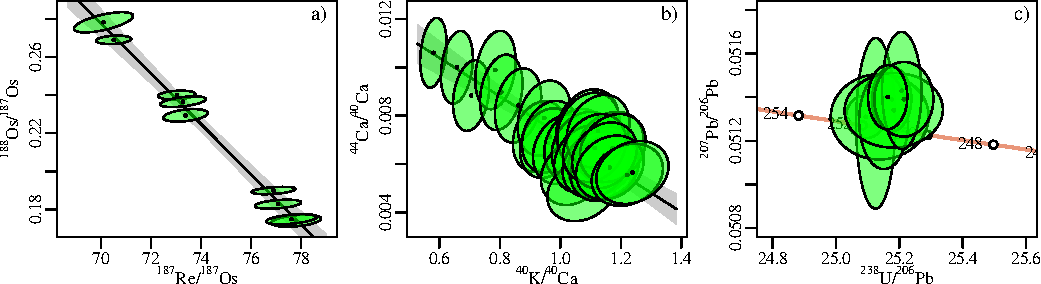
\includegraphics[width=\textwidth]{../figures/inverrorcorrelation_edited.pdf}
\begingroup
\captionof{figure}{ Recasting the data of
  Figure~\ref{fig:errorcorrelation} into an inverse ratio form reduces
  the error correlations for the Re--Os, K--Ca and U--Pb data.\\}
\label{fig:inverrorcorrelation}
\endgroup

Given a data table of conventional ratios ($X=x/z$ and $Y=y/z$), it is
possible to calculate the inverse ratios ($X'=x/y$ and $Y'=z/y$),
their uncertainties ($s[X']$ and $s[Y']$) and error correlations
($r[X',Y']$) using the following equations:

\begin{equation}
  \begin{cases}
    X' = \frac{X}{Y} \\
    Y' = \frac{1}{Y} \\
    \left(\frac{s[X']}{X'}\right)^2 =
    \left(\frac{s[X]}{X}\right)^2 -
    2 r[X,Y]\left(\frac{s[X]}{X}\right)\left(\frac{s[Y]}{Y}\right) +
    \left(\frac{s[Y]}{Y}\right)^2 \\
    \left(\frac{s[Y']}{Y'}\right)^2 = \left(\frac{s[Y]}{Y}\right)^2 \\
    r[X'Y'] =
    \left(\frac{X'}{s[X']}\right)
    \left[
    \left(\frac{Y}{s[Y]}\right) -
    r[X,Y]\left(\frac{X}{s[X]}\right)
    \right]
  \end{cases}
  \label{eq:transformation}
\end{equation}

This transformation is perfectly symmetric in the sense that it can
also be used to convert inverse isochron ratios to conventional
ones. To do this, it suffices to swap $X'$ and $Y'$ for $X$ and $Y$
and vice versa. \texttt{IsoplotR} carries out these conversions on the
fly. So if a data file provides the isotopic composition as
conventional ratios, then it is possible to plot the data as inverse
ratios without worrying about the details of the conversion.

\section{Linear regression}
\label{sec:regression}

As briefly discussed in Chapter~\ref{ch:intro2PD}, isochrons are an
important instrument of high precision, high accuracy geochronology.
Given several aliquots from a single sample, they allow the
non-radiogenic component of the daughter nuclide to be quantified and
separated from the radiogenic component. A conventional isochron is
obtained by fitting a straight line through the conventional isochron
ratios introduced in Section~\ref{sec:errorcorrelations}. The slope
and intercept then yield the radiogenic daughter-parent ratio and the
non-radiogenic daughter composition, respectively
\citep{nicolaysen1961}. In its simplest form, isochrons are fitted by
ordinary least squares regression.\\

Consider a set of $n$ bivariate data points $x =
\{x_1,x_2,\ldots,x_n\}$ and $y = \{y_1,y_2,\ldots,y_n\}$.  The best
fit straight line through these data can be found by minimising the
sum of the squared residuals:
\begin{equation}
  S = \sum\limits_{i=1}^{n}\left( y_i - a - b x_i \right)^2
  \label{eq:S}
\end{equation}

\noindent where $a$ is the intercept and $b$ the slope. However this
method does not take into account the analytical uncertainties of the
isotopic ratio measurements. In a first step, let us consider the
situation where only the dependent variable ($y$) is affected by
significant analytical uncertainty, and let $s[y] =
\{s[y_1],s[y_2],\ldots,s[y_n]\}$ be the corresponding standard
errors. Then the least squares criterion can be modified to create a
weighted regression algorithm:
\begin{equation}
  S_w = \sum\limits_{i=1}^{n}\left( \frac{y_i - a - b x_i}{s[y_i]} \right)^2
  \label{eq:Swtd}
\end{equation}

Alternatively (and equivalently), the best fit line can also be
obtained by maximising the log-likelihood:
\begin{equation}
  \mathcal{LL} = - \sum\limits_{i=1}^{n} \ln\left(2 \pi s[y_i] \right)
  - \frac{S_w}{2}
  \label{eq:L}
\end{equation}

To illustrate the usefulness of the weighted regression algorithm,
consider a simple three-point example. Let $\boldsymbol{x} = \{10, 20,
40\}$ and $\boldsymbol{y} = \{20,30,50\}$ be the \emph{true} x- and
y-coordinates of the three points\footnote{In the remainder of this
  paper, bold face will be used to mark the true values, whereas
  normal face will be used to mark the actual measurements (i.e. the
  true value plus some random analytical uncertainty).}. It is easy to
see that these fall on a perfect line with intercept $\boldsymbol{a} =
10$ and slope $\boldsymbol{b} = 1$. Let $s[\boldsymbol{y}] =
\{1,1,10\}$ be the analytical uncertainties of \textbf{y}, so that the
third point is ten times less precise than the first two. Further let
$y = \{20,30,60\}$ be a random realisation of \textbf{y}.  Then the
best ordinary least squares fit through $x = \boldsymbol{x}$ and $y$
has an intercept of $a = 5.0$ and a slope of $b = 1.36$. This poor
result is strongly influenced by the third, least precise data
point. Subjecting the same dataset to weighted linear regression
yields $a = 9.4$ and $b = 1.04$. This is a far more accurate result
(Figure~\ref{fig:regression}.a).\\

In isochron regression, it is typical for not only $y$ but also $x$ to
be affected by analytical uncertainty. In this case, the best fit line
can be found by modifying the likelihood function
\citep{titterington1979, york1969, york2004}:

\begin{equation}
  \mathcal{LL}_y = 
  -\frac{1}{2} \sum\limits_{i=1}^{n}
  \ln\left(2 \pi |\Sigma_i| \right)
  -\frac{1}{2} \sum\limits_{i=1}^{n}
  \left[X_i-\hat{X}_i\right]^T
  \Sigma_i^{-1}
  \left[X_i-\hat{X}_i\right]
  \label{eq:Ly}
\end{equation}

\noindent where

\begin{equation}
  X_i = \left[
    \begin{array}{@{}c@{}}
      x_i\\
      y_i\\
    \end{array}
    \right]
  \mbox{~,~}
  \hat{X}_i = \left[
    \begin{array}{@{}c@{}}
      \hat{x}_i \\
      a + b \hat{x}_i
    \end{array}
    \right]
  \mbox{~and~}
  \Sigma_i = \left[
    \begin{array}{@{}cc@{}}
      s[x_i]^2 & s[x_i,y_i] \\
      s[x_i,y_i] & s[y_i]^2
    \end{array}
    \right]
\end{equation}

\noindent where $\hat{x}_i$ are the \emph{estimated} values of
$\mathbf{x}_i$ for any value of $a$ or $b$. $s[x_i,y_i]$ is the
covariance of the $i$\textsuperscript{th} measurement's x- and
y-uncertainties. To illustrate the importance of these covariance
terms, consider a second three-point example:

\begin{center}
\begin{tabular}{cccccc}
  $i$ & \textbf{x} & $s[\boldsymbol{x}]$ & \textbf{y} &
  $s[\boldsymbol{y}]$ & $s[\boldsymbol{x}_i,\boldsymbol{y}_i]$ \\
  \hline
  1 & 10 & 1 & 20 & 1 & 0.9 \\
  2 & 20 & 1 & 30 & 1 & 0.9 \\
  3 & 30 & 1 & 40 & 1 & -0.9
\end{tabular}
\end{center}

\noindent which again defines a straight line with intercept $a = 10$
and slope $b = 1$. Let $x = \{10,20,28\}$ and $y = \{20,30,42\}$ be a
random realisation of \textbf{x} and \textbf{y}. Suppose that we
ignored or did not know the covariance terms. In that case the
ordinary and weighted regression algorithms would yield the same
outcome because all the samples have the same standard errors ($s[x_i]
= s[y_i] = 1$ for all $i$). The resulting intercept and slope would
then be $a = 7.2$ and $b = 1.21$. However, if we do take into account
the covariances, then the maximum likelihood algorithm yields $a =
9.3$ and $b = 1.05$, which is much closer to the true values of
$\boldsymbol{a} = 10$ and $\boldsymbol{b} = 1$
(Figure~\ref{fig:regression}.b).

\begin{center}
\noindent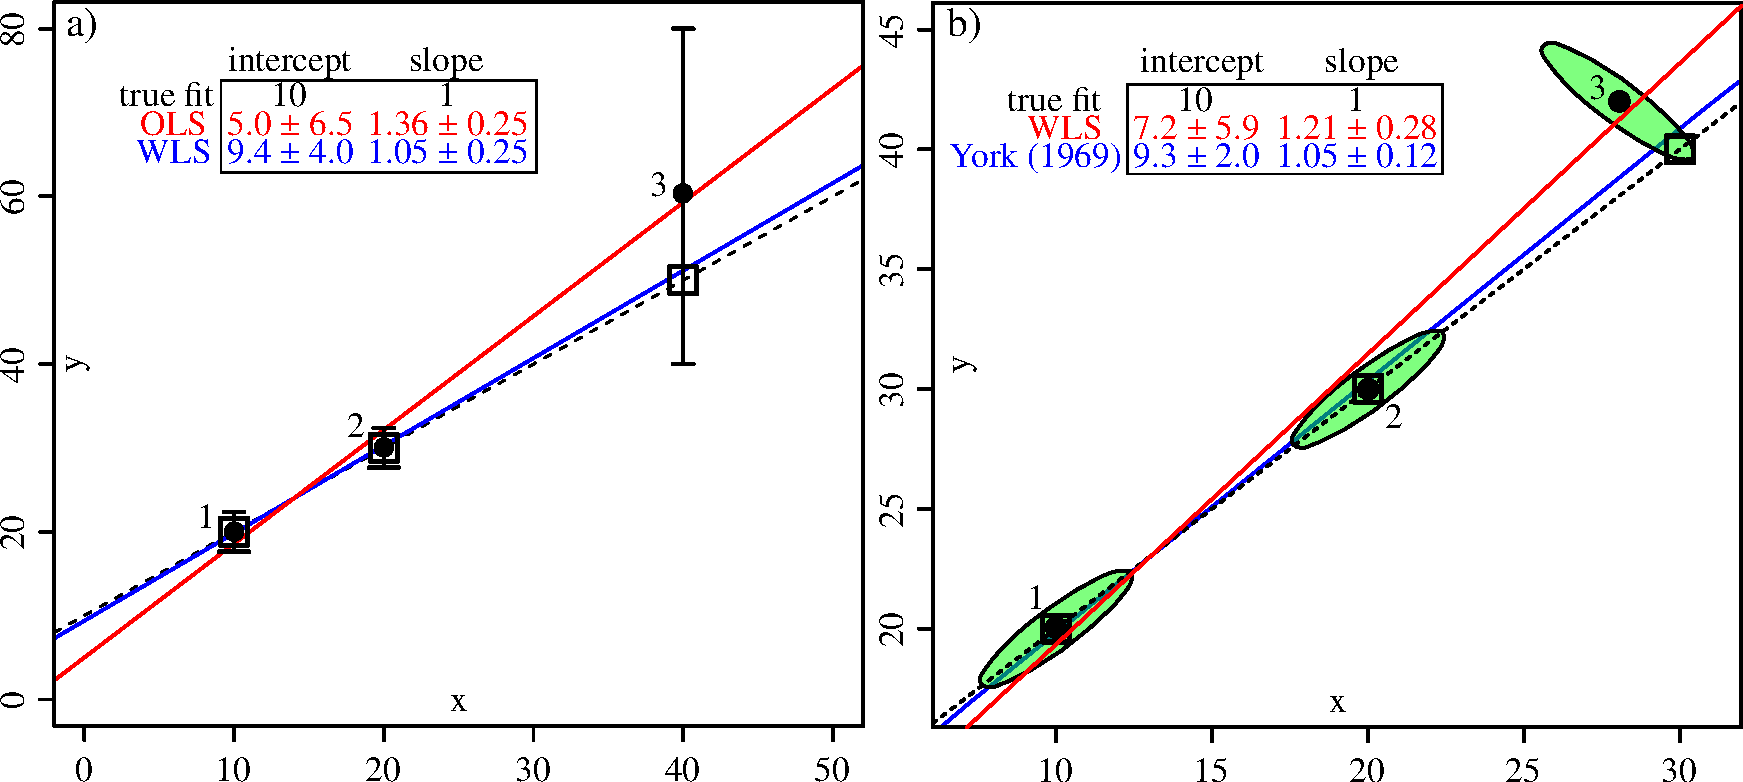
\includegraphics[width=.85\textwidth]{../figures/regression.pdf}
\captionof{figure}{Illustration of the benefits of error-weighted
  linear regression.  The black squares mark the true
  (x,y)-coordinates of three samples drawn from a (dashed) line with
  intercept $\boldsymbol{a} = 10$ and slope $\boldsymbol{b} = 1$. The
  black dots mark random realisations of these samples, given Gaussian
  uncertainties with uncertainties shown as 95\% confidence bars or
  ellipses. a) three samples with analytical uncertainty in the
  y-variable only. The ordinary least squares fit ignoring these
  uncertainties is shown in red ($a = 5.0, b = 1.36$), the weighted
  least squares fit in blue ($a = 9.4, b = 1.04$). b) three samples
  with correlated uncertainties in both the x- and y-variable.
  Ignoring the error correlations yields the red fit ($a = 7.2, b =
  1.21$). Accounting for the error correlations produces the blue fit
  ($a = 9.3, b = 1.05$).}
\label{fig:regression}
\end{center}

The extent to which the observed scatter in the data around the best
fit isochron line can be explained by the analytical uncertainties can
be assessed using a chi-square test, in nearly exactly the same manner
as described for the weighted mean in Section~\ref{sec:mswd}. In the
case of linear regression, the chi-square statistic is defined as:
\begin{equation}
  \chi_{stat}^2 = \sum\limits_{i=1}^{n} \left[X_i - \hat{X}_i\right]^T
  \Sigma_i^{-1} \left[X_i - \hat{X}_i\right]
  \label{eq:Chi2}
\end{equation}

\noindent in which we recognise the second term of
Equation~\ref{eq:Ly}, which is the matrix formulation of the sum of
squares. We can compare this value with a chi-square distribution with
$df = (k-1)(n-2)$ degrees of freedom, where $k$ is the dimensionality
of the linear fit. Thus, for bivariate regression, $df=n-2$ and for
trivariate linear regression, $df=2n-4$. The MSWD is again defined as
\[
MSWD = \chi^2_{stat}/df
\]

In complete analogy to the weighted mean of Section~\ref{sec:mswd},
the MSWD can be used to assess whether the scatter of the data falls
within the range expected from the analytical uncertainties, or
whether the data if over- or underdispersed. An in the case of
overdispersion, there are three ways (`models') to deal with this
overdispersion:

\begin{enumerate}
\item model-1: inflate the analytical uncertainties by a factor
  $\sqrt{MSWD}$;
\item model-2: ignore the uncertainties and fall back to ordinary
  least squares regression;
\item model-3: attribute the overdispersion to a second source of
  uncertainty in the intercept or slope of the line.
\end{enumerate}

\noindent\begin{minipage}[t]{.4\textwidth}
\strut\vspace*{-\baselineskip}\newline
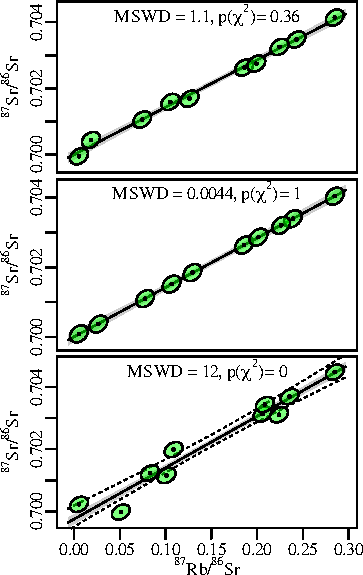
\includegraphics[width=\textwidth]{../figures/isochronMSWD.pdf}
\end{minipage}
\begin{minipage}[t]{.6\textwidth}
  \vspace{-10pt} \captionof{figure}{Three different synthetic Rb--Sr
    data sets shown as conventional isochron plots. The analytical
    uncertainties are shown as 95\% error ellipses. The grey band
    represents a 95\% confidence envelope for the best fit line using
    the \citet{york1969} algorithm. Each of the data sets consists of
    10 aliquots that are affected by a combination of analytical and
    geological dispersion. The relative importance of these two
    sources of scatter can be assessed using the mean square of
    weighted deviates (MSWD) and the p-value of the chi-square
    test. The case where MSWD$\approx{1}$ is the easiest to interpret:
    it means that the scatter of the data around the best fit line can
    be completely explained by the analytical uncertainty. The case
    where MSWD$<{1}$ may seem like a good outcome but it is in fact a
    bad one because it indicates that there may be a problem with the
    error propagation. A high p-value or low MSWD may happen once but
    red flags should go up if all samples in a study show this type of
    behaviour. Finally the case where MSWD$>{1}$ is not good or bad
    but `interesting'. The dashed line marks the `overdispersion'
    estimated by a model-3 regression.}
  \label{fig:isochronMSWD}
\end{minipage}

\section{Confidence intervals}
\label{sec:CI}

Figure~\ref{fig:2sigma} showed that approximately 95\% of the normal
distribution falls within two standard deviations of the mean. Thus,
if we know that $x$ was drawn from a normal distribution with standard
deviation $\sigma$ and an unknown mean $\mu$, then 95\% of all $x$-values
are expected to fall in the interval
\[
\mu - 2\sigma \leq x \leq \mu + 2\sigma
\]

Subtracting $x$ and $\mu$ from all terms:
\[
-x - 2\sigma \leq -\mu \leq -x + 2\sigma
\]

Multiplying with $-1$:
\[
x + 2\sigma \geq \mu \geq x - 2\sigma
\]

\noindent which gives rise to the following 95\% confidence interval
for $\mu$:
\[
\mu \in \{ x \pm 2\sigma \}
\]

\noindent which gives rise to the popular `2-sigma' confidence
interval.  Chapter~\ref{ch:error-propagation} showed that the standard
error of the mean is given by
\[
s[\bar{x}] = s[x]/\sqrt{n}
\]

One might be tempted to assume that $\bar{x} \pm 2 s[\bar{x}]$
constitutes a 95\% confidence interval for $\mu$. However, this would
be incorrect because $\bar{x}$ does \emph{not} follow a normal
distribution. To construct a 95\% confidence for $\mu$ based on
$\bar{x}$, we first define the `t-statistic' as follows:
\begin{equation}
  \mathbf{t} = \frac{\bar{x}-\mu}{s[\bar{x}]}
  \label{eq:tstat}
\end{equation}

\noindent where $\mathbf{t}$ is written in bold to avoid confusion
with the geological age $t$ used elsewhere in these
notes. $\mathbf{t}$ follows a `t-distribution with $n-1$ degrees of
freedom'. By definition, the 95\% confidence interval is the
collection of all those values of $\mu$ for which
\[
t_{df,\alpha/2} \leq \mathbf{t} \leq t_{df,1-\alpha/2}
\]

\noindent where $t_{df,\alpha/2}$ and $t_{df,1-\alpha/2}$ are the
$\alpha/2$ and $(1-\alpha/2)$ quantiles of a t-distribution with $df$
degrees of freedom, respectively.  Hence:
\[
t_{df,\alpha/2} \leq \frac{\bar{x} - \mu}{s[\bar{x}]} \leq t_{df,1-\alpha/2}
\]

\noindent Rearranging:
\[
\bar{x} - t_{df,\alpha/2}s[\bar{x}] \geq \mu \geq
\bar{x} - t_{df,1-\alpha/2}s[\bar{x}]
\]

\noindent Because the t-distribution is symmetric around zero, we can also write:
\[
t_{df,1-\alpha/2} = -t_{df,\alpha/2}
\]

\noindent Hence
\[
\bar{x} + t_{df,\alpha/2}s[\bar{x}] \leq \mu \leq \bar{x} - t_{df,\alpha/2}s[\bar{x}]
\]

\noindent or
\begin{equation}
  \mu \in \left\{\bar{x} \pm t_{df,\alpha/2}s[\bar{x}]\right\}
  \label{eq:tci}
\end{equation}

For large samples (and, hence, degrees of freedom), the t-statistic is
approximately equal to 2. But for small samples, it is greater than 2
and the 95\% confidence interval for $\mu$ is wider as a consequence.

\noindent\begin{minipage}[t][][b]{.6\textwidth}
  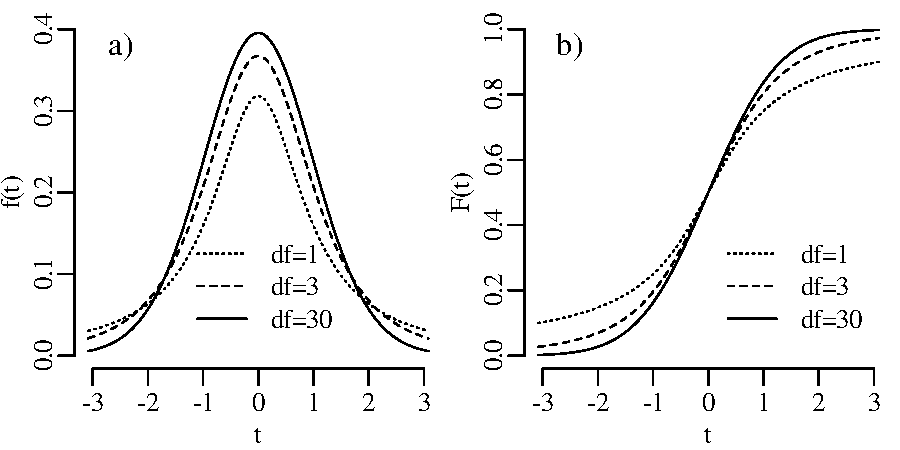
\includegraphics[width=\textwidth]{../figures/tdof.pdf}\\
\end{minipage}
\begin{minipage}[t][][t]{.4\textwidth}
  \captionof{figure}{a) pdfs and b) cdfs of the t-distribution for
    three different degrees of freedom ($df$). For small sample sizes
    (low $df$), the t-distribution has long tails towards low and high
    values. With increasing sample size, the tails become shorter and
    the t-distribution sharper. When $df>30$, the t-distribution is
    indistinguishable from a standard normal distribution with $\mu=0$
    and $\sigma=1$.}
  \label{fig:tdof}
\end{minipage}

\texttt{IsoplotR} reports the age uncertainties in the following
form:

\[
t = \hat{t} \pm x \mid y (\mid z)
\]

\noindent where

\begin{description}
\item[$\hat{t}$] is the age estimate
\item[$x$] is the standard error of $\hat{t}$
\item[$y$] $= t_{df,1-\alpha/2} \times x$ is the 95\% confidence interval for
  $\hat{t}$
\item[$z$] $= \sqrt{MSWD} \times y$ is the 95\% confidence interval for
  $\hat{t}$ adjusted for overdispersion. This value is only reported
  for model-1 fits when the p-value of the chi-square test is less
  than 0.05.
\end{description}

\noindent\begin{minipage}[t][][b]{.6\textwidth}
  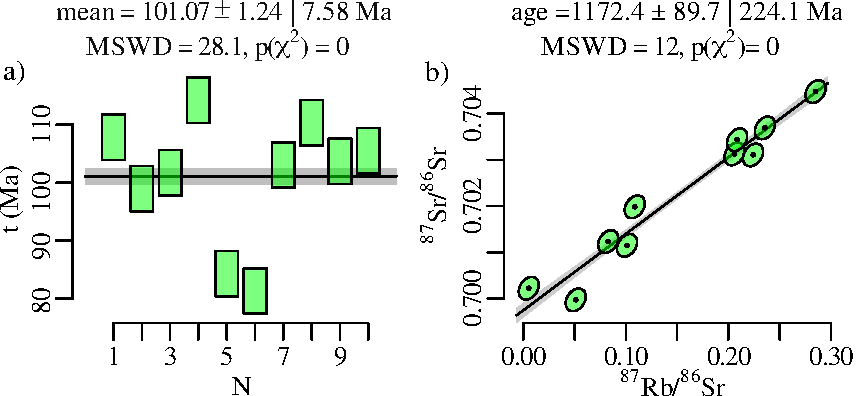
\includegraphics[width=\textwidth]{../figures/model-1.pdf}\\
\end{minipage}
\begin{minipage}[t][][t]{.4\textwidth}
  \captionof{figure}{a) weighted mean (Figure~\ref{fig:wtdmeanMSWD}c)
    and b) Rb--Sr isochron (Figure~\ref{fig:isochronMSWD}c) regression
    using a model-1 fit. The legend reports the best fit age and
    uncertainties reported as standard errors, and 95\% confidence
    intervals with and without overdispersion.  }
  \label{fig:model-1}
\end{minipage}

With regards to error propagation, it is important to make a
distinction between \textbf{random} and \textbf{systematic} sources of
uncertainty. Random uncertainties can be reduced to arbitrarily low
levels by averaging an arbitrarily large number of aliquots. In
contrast, systematic uncertainties impose absolute limits on the
precision of geochronological dates.  For example, no absolute age
determination can be more precise than the decay constants
involved. Similarly, for dating methods such as
\textsuperscript{40}Ar/\textsuperscript{39}Ar or fission tracks, no
sample date can be more precise than the $J$ and $\zeta$ calibration
factors, respectively.\\

When solving Equation~\ref{eq:wtdmean}, \texttt{IsoplotR} only
incorporates the random sources of uncertainty into $s[t_i]$.  If the
user wishes to include the systematic uncertainties as well, then this
is done by first computing the isotopic composition corresponding to
the weighted mean age (and its uncertainty), and then re-propagating
the analytical uncertainty of the weighted mean age, this time
including the decay or calibration constant uncertainties.\\

Note that this procedure is unable to handle the systematic
uncertainties associated with stable isotope ratios, molar masses
etc. Those comparably small uncertainties demand a different approach
in which not the ages but the isotopic data are averaged.  Doing so
would require the addition of new input formats that can trace error
correlations between samples (Chapter~\ref{sec:future}). It would also
require the development of a new generation of low-level
data-processing software \citep{vermeesch2015b,mclean2016}.

\noindent\begin{minipage}[t]{.33\linewidth}
\strut\vspace*{-\baselineskip}\newline
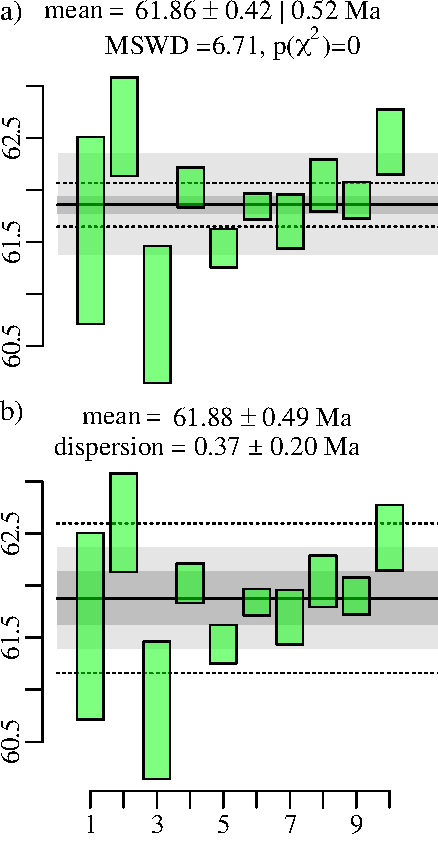
\includegraphics[width=\textwidth]{../figures/WtdMeanModel1vsRandomEffects.pdf}
\end{minipage}
\begin{minipage}[t]{.2\linewidth}
\end{minipage}
\begin{minipage}[t]{.65\linewidth}
  \captionof{figure}{ a) ordinary weighted mean (model-1) and b)
    random effects model (model-3) of the same dataset. The dark and
    light grey bands show the 95\% confidence intervals the weighted
    mean without and with external uncertainties, respectively. The
    dashed lines have a different meaning for the two plots. For panel
    a), they mark the 95\% confidence interval with overdispersion
    (i.e., the dark grey band augmented with a factor
    $\sqrt{\mbox{MSWD}}$). For panel b), they mark the 95\% confidence
    limits of a normal distribution whose mean equals the weighted
    mean from the random effects model, and whose standard deviation
    equals the dispersion parameter ($\omega$).}
  \label{fig:WtdMeanModel1vsRandomEffects}
\end{minipage}


\printbibliography[heading=subbibliography]

\end{refsection}
